
\section{Overlapping Shapes}
As previously mentioned the PCAL functions as a hodoscope, allowing determination of the x,y position of a hit within a resolution determined by the overlap of the strips from each of the U,V,W layers.  One can think of dividing each PCAL module into bins based on the 
overlapping shapes. The overlap shapes/pixels are of two types: a 3-strip pixel, which is a shape formed when all three views are superimposed together, and a 2-strip pixel formed from the overlap of two strips where the strips are
part of different views.  Maps of different overlap conditions are shown in Fig.~\ref{fig:PCAL_overlap}.
\textcolor{red}{The current analysis extracts the attenuation calibration based on 2-strip pixels only.}


\begin{figure}[h]
  \centering
  \begin{subfigure}[b]{0.45\textwidth}
  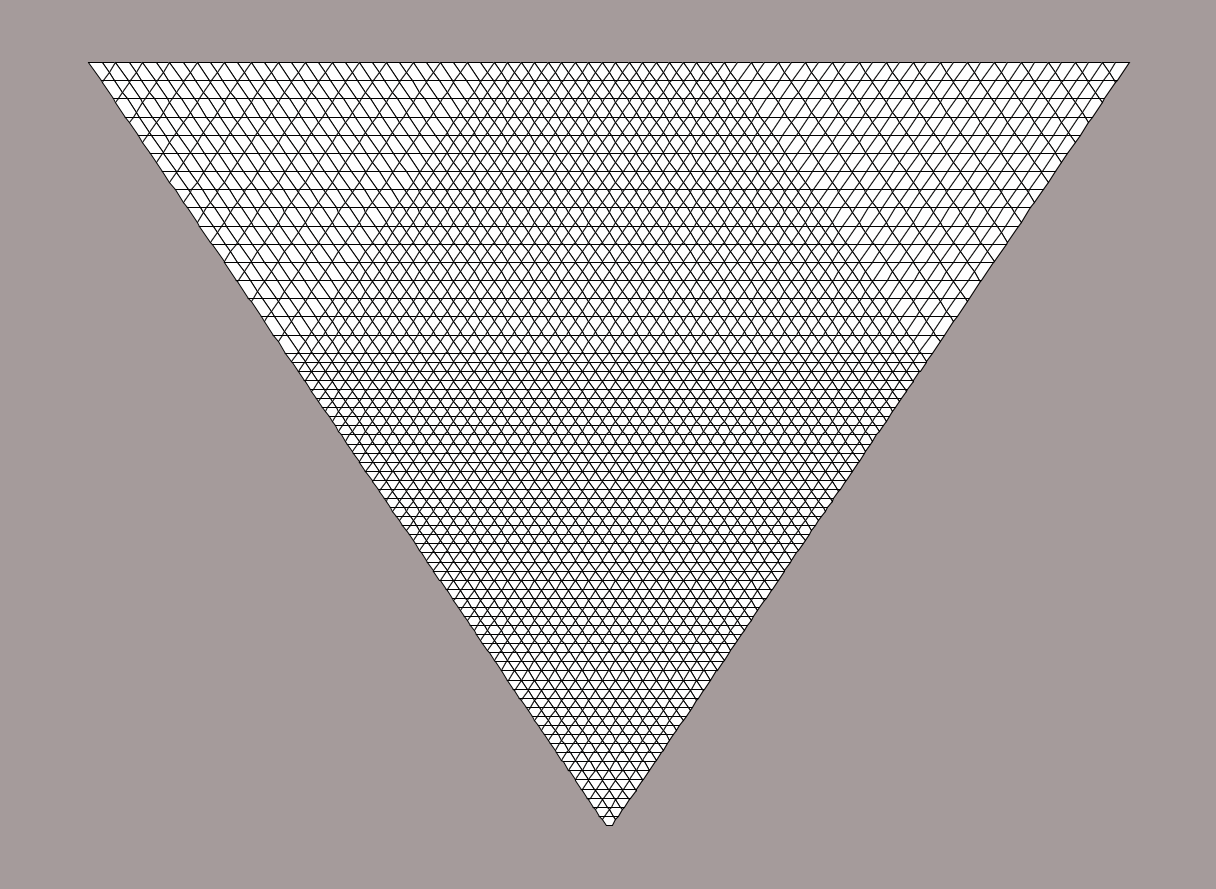
\includegraphics[width= 3in, keepaspectratio = true]{PCAL_pixel_screenshot}
  \caption{UVW overlap.}
  %\label{fig:PCAL_pixel_screenshot}
  \end{subfigure}
  ~
  \begin{subfigure}[b]{0.45\textwidth}
  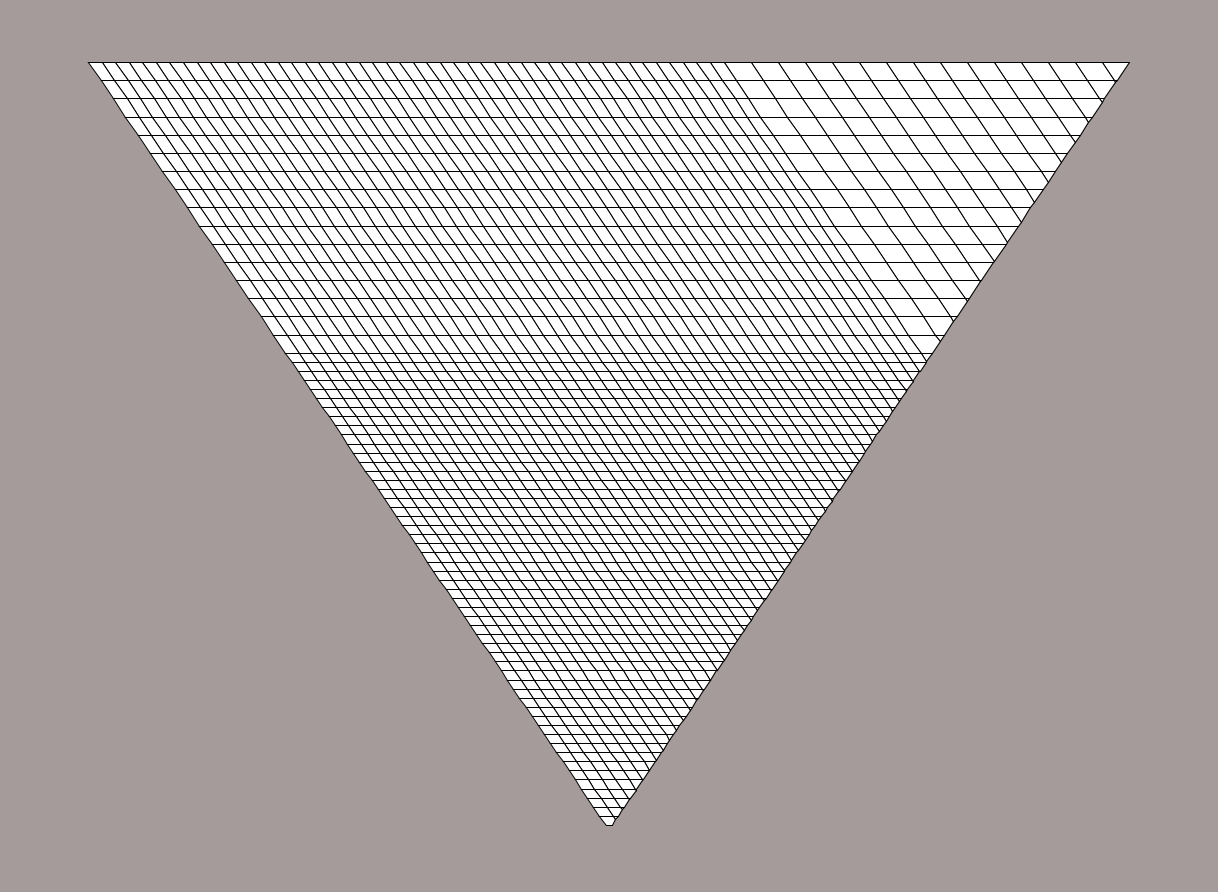
\includegraphics[width= 3in, keepaspectratio = true]{PCAL_UW_screenshot}
  %\caption{$M_{\pi^{+}\pi^{-}}$}
  %\label{fig:geomfig3b}
  \caption{UW overlap.}
  %\label{fig:PCAL_UW_screenshot}
  \end{subfigure}

  \begin{subfigure}[b]{0.45\textwidth}
  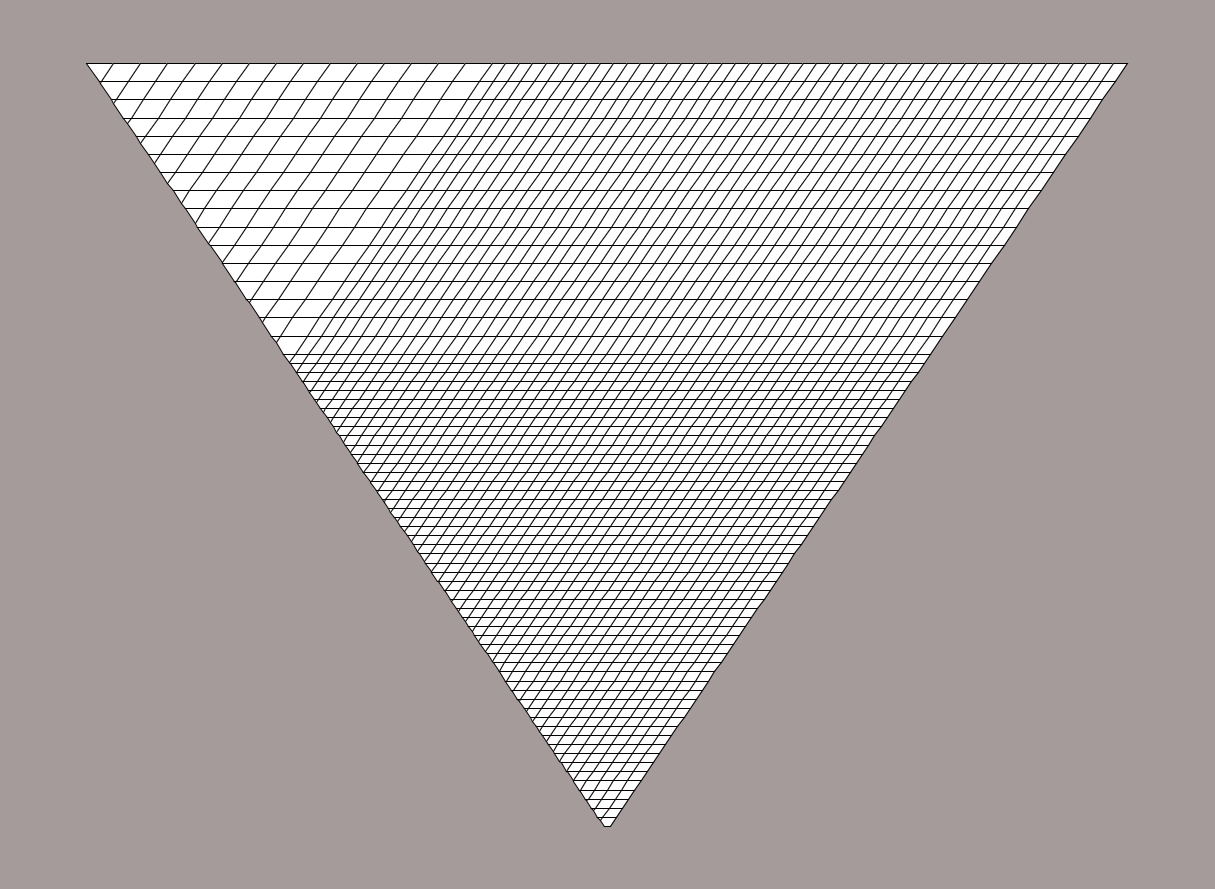
\includegraphics[width= 3in, keepaspectratio = true]{PCAL_UV_screenshot}
  %\caption{$M_{\pi^{+}\pi^{-}}$}
  %\label{fig:geomfig3b}
  \caption{UV overlap.}
  %\label{fig:PCAL_UV_screenshot}
 \end{subfigure}
  ~
  \begin{subfigure}[b]{0.45\textwidth}
  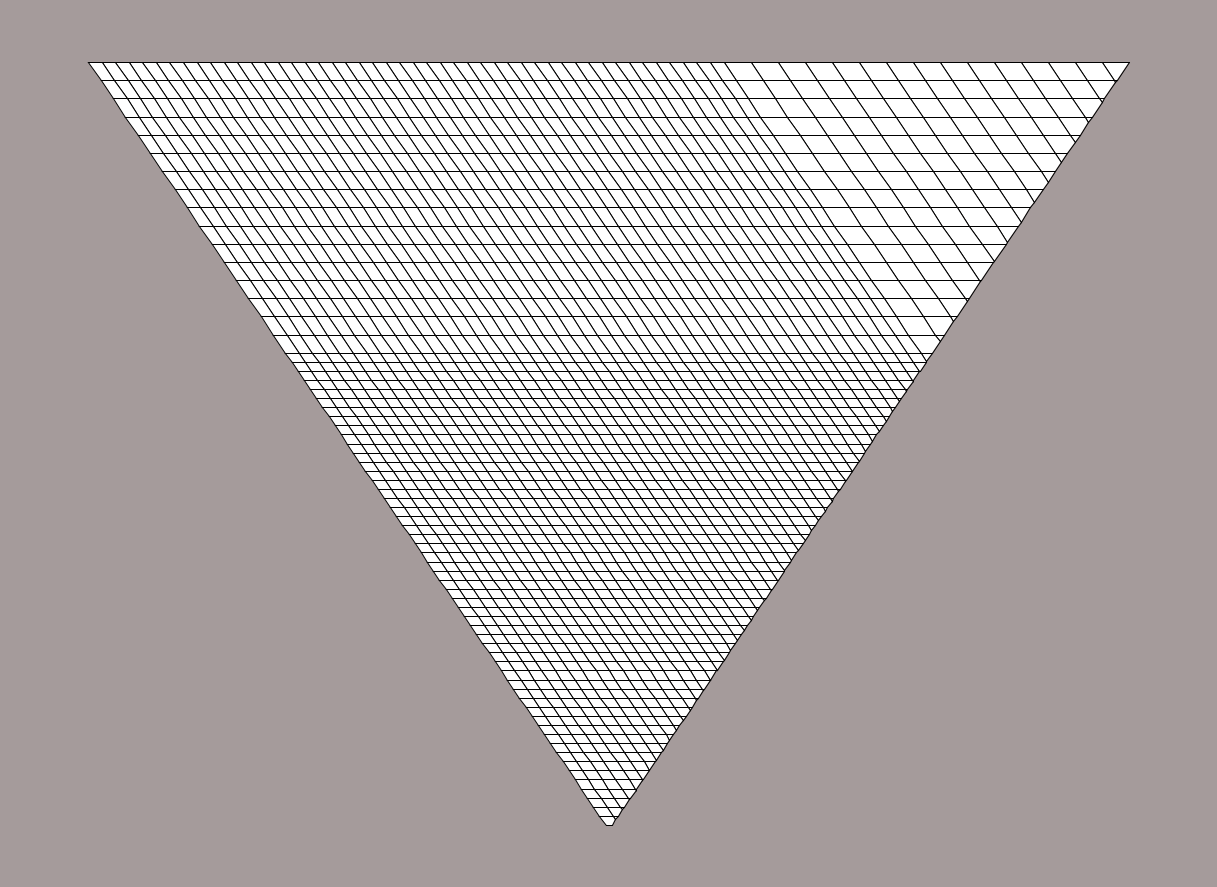
\includegraphics[width= 3in, keepaspectratio = true]{PCAL_WU_screenshot}
  \caption{WU overlap.}
  %\label{fig:PCAL_WU_screenshot}
  \end{subfigure}
  ~
  \caption{Shown are the different ways overlaps can be considered in a single PCAL module.}
  \label{fig:PCAL_overlap}
\end{figure}
\FloatBarrier


